I vores program er der 3 forskelige thresholdt som påvirker hvordan
metoden analysere billedet. Marginens brade, afvigelsen af farven i
floodfill og afvigelsen i farven i kandtdetection. Alle 3 thresholdt er
blevet introduseret i deres respektive afsnit, men ingen konkreade tal
er opgivet. I dette afsnit vil vi opgive de tal, samt en forklaring på
hvorfor vi har valt lige de tal.

\subsection{Marginens brede}
Vi regner marginens brade $MB$ ud fra en procent af billedets brade og
højde. I afsnitte \ref{opdeling_af_billeder.tex} kom vi frem til en
usikkerhed på $2.1 \%$ i vores udregninger, så hvores $MB$ skal minst
være på $2.1 \%$. Ud over det er den minimale forskel på 2 snit,
forskellen mellem det gyldne snit og $\frac{2}{3}$, som vi udregnet i
section \ref{opdeling_af_billeder-tex} til maximal at have en $MB$ på
$2.43$ få at margin ikke krysset. Så $MB \in [2.1, 2.43]$ og vi har valt
at sætte $MB = 2.4$, da vi så kan tage højde for udforsende usikker
heder som i ikke har opdaget inu XXX(er det en dog nok forklaring).

\subsection{Afvigelsen af farver i floodfill}

lo,lu = 4,4
lo,lu = 5,5
lo,lu = 6,6
lo,lu = 3,3

\subsection{Afvigelsen af farver i kandtdetection}
Vores ubberste mål med brugen af kandtdetection er af finde en kand rundt om de ragioner som vi menner er interasante, og undgå de kanter som ligger inde i ragioner. alt det kan ikke altid opfyldes, men vi kan komme så tæt på et kompromi mellem en perfect kant rund om ragion og ingen kanter inde i ragion som mulige. Dette gøres ved at ændre 2 tærskelværdiger i kantdetection ud for opsavationer som vi har taget på billederne i forvejen. Vi har valt at dele billederne som vi opsavere op i 9 kategorier, som vi vil gemmengå og komme inde på vores valg

\subsubsection{sammenlininger}
Vi har set på et XX(hvormange) andtal malerier og har fundet de tærskelværdiger som vi menner passer best på billedet. Vi vil ilustrere framgange måden på maleriet \ref{kDetalier}, på maleriet kan man se der er mange farver og har masser af detaliger i sig. Måden vi har arbejdet os frem på er, ved at se på malleriet med tærskelværdig $[0,0],[100,100]......[900,900],[1000,1000]$ se figur \ref{allesammen1} og \ref{allesammen2}, og finde det intervalder hvor malerriet ikke har mistet nogle af sine kanter inu, men vil det, i næste intervalg, i ilustration vudere vi det til billedet \ref{300-300}, da billedet \ref{400-400} har mistet få meget af de kanter som vi gerne vil beholde. Som man kan se befinde tærskelværdien som vi gerne vil finde fram til fra $[300,300]$ og frem. Ved at sætte den anden tærskel værdig op lidt af gangen kan vi igen få en række billeder at vælje imellem, få at få det beste resultat, se sammenliningerne i figur \ref{allesammen3}. som man kan se begynder det er være svær at skeldne figurene i \ref{300-850} og der er lidt for mange kanter i \ref{300-700}, så vi har valdt at tage tærskeværdigerne $[300,750]$ få dette billedet. Man kunne god gå længer ned og se om tærskeværdig $[300,745]$ passet bedre, men XXX(). Det maleri vi lige har brugt er ikke serlige representativ for helle vores malleri database, så vi har taget en række billeder og brugt samme metode på dem og kommer frem til en midel tærskelværdig, jeg viser her en lille udsnit af dem, se figur %\ref{1},
%\ref{2},\ref{3},\ref{4},\ref{5},\ref{6},\ref{7} og \ref{8}
\begin{figure}[!h]
    \centering
    \subfloat[100,100]{
        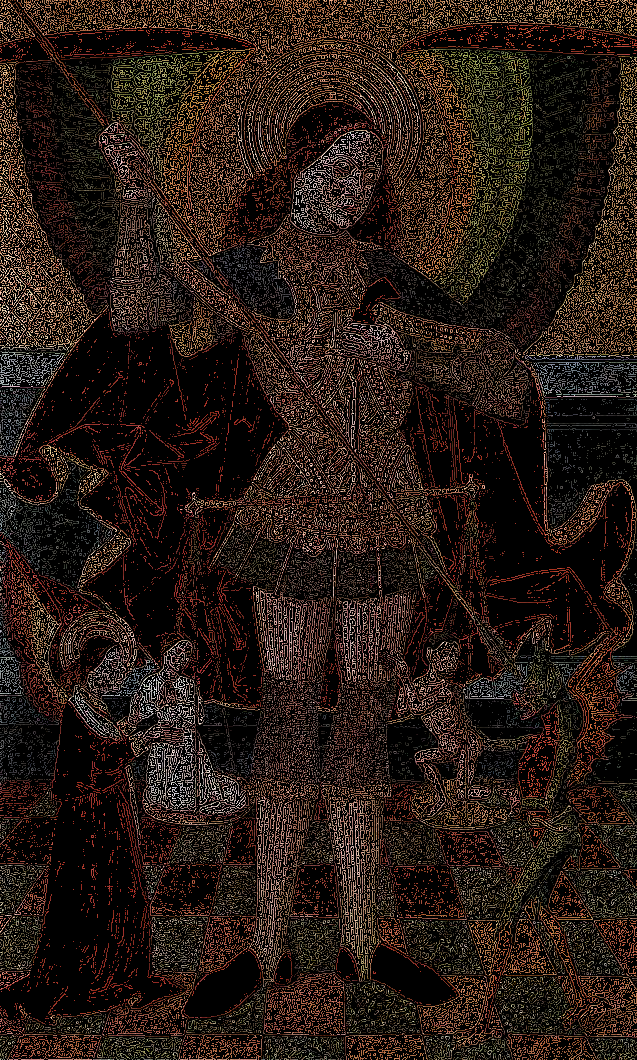
\includegraphics[angle=0,width=0.45\textwidth]{afsnit/afprovning/billeder/thressholds/krafitige_farver/krafite_detalier/1_iteration/100-100.png}
        \label{100-100}}\hspace{1em}
    \subfloat[200,200]{
        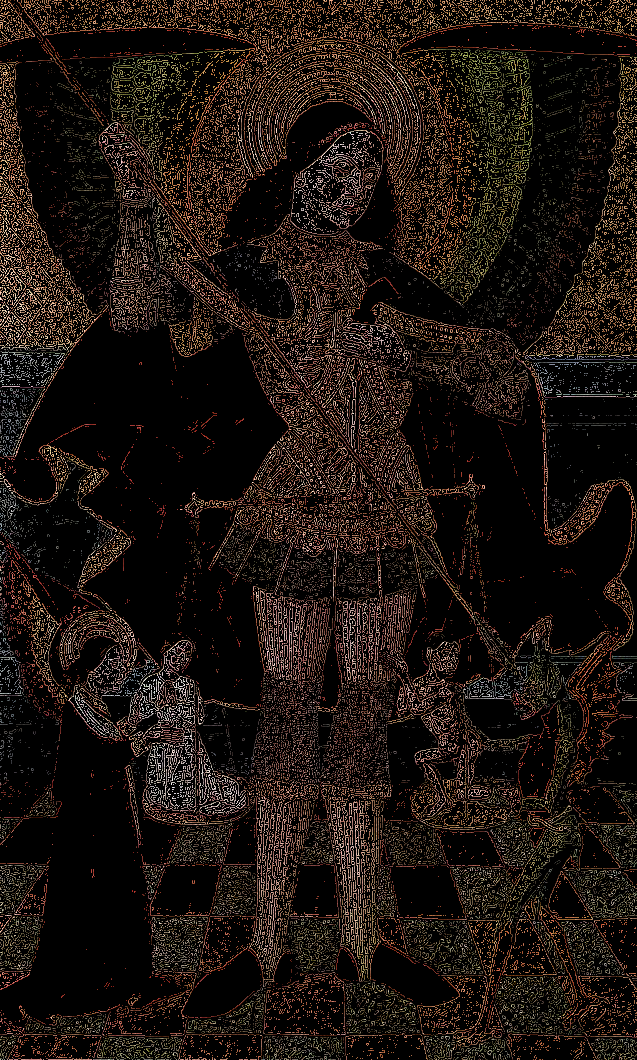
\includegraphics[angle=0,width=0.45\textwidth]{afsnit/afprovning/billeder/thressholds/krafitige_farver/krafite_detalier/1_iteration/200-200.png}
        \label{200-200}}\\
    \subfloat[300,300]{
        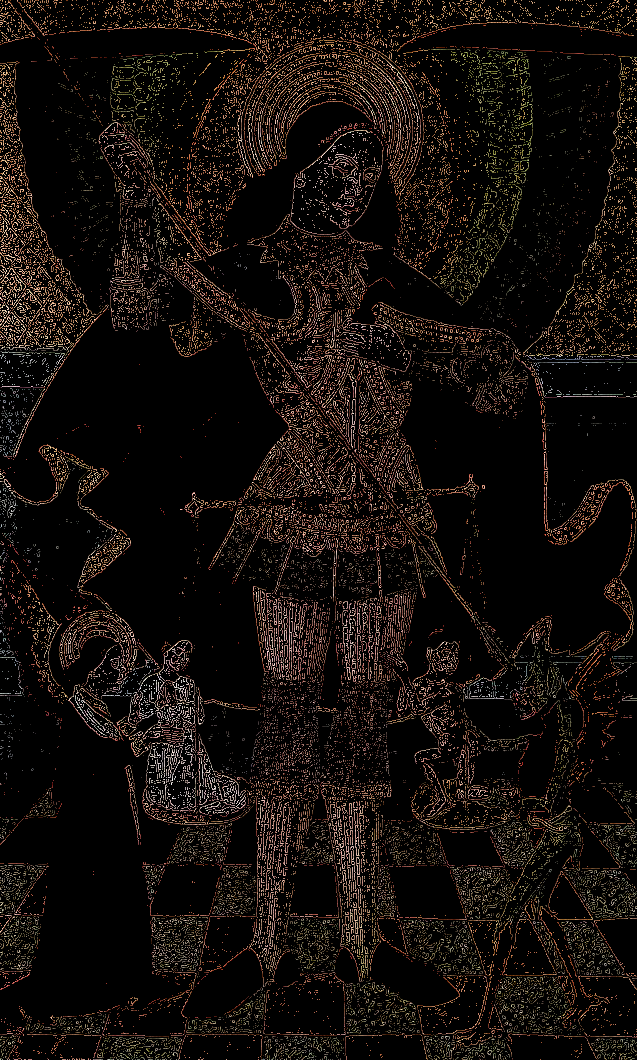
\includegraphics[angle=0,width=0.45\textwidth]{afsnit/afprovning/billeder/thressholds/krafitige_farver/krafite_detalier/1_iteration/300-300.png}
        \label{300-300}}\hspace{1em}
    \subfloat[400,400]{
        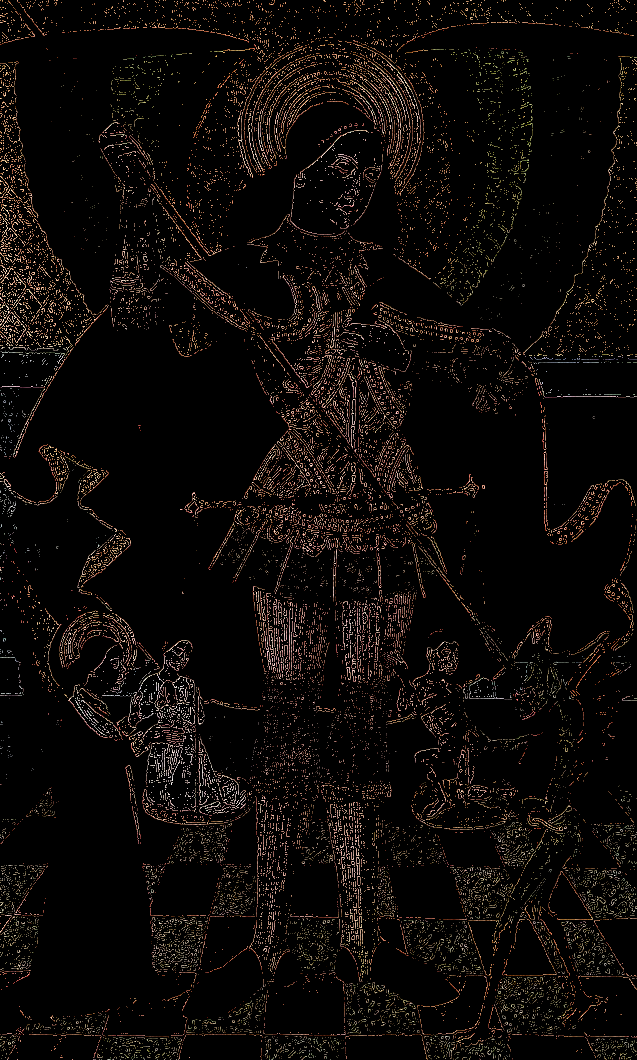
\includegraphics[angle=0,width=0.45\textwidth]{afsnit/afprovning/billeder/thressholds/krafitige_farver/krafite_detalier/1_iteration/400-400.png}
        \label{400-400}}\\
     \label{allesammen1}
\end{figure}
\begin{figure}[!h]
	    \subfloat[500,500]{
        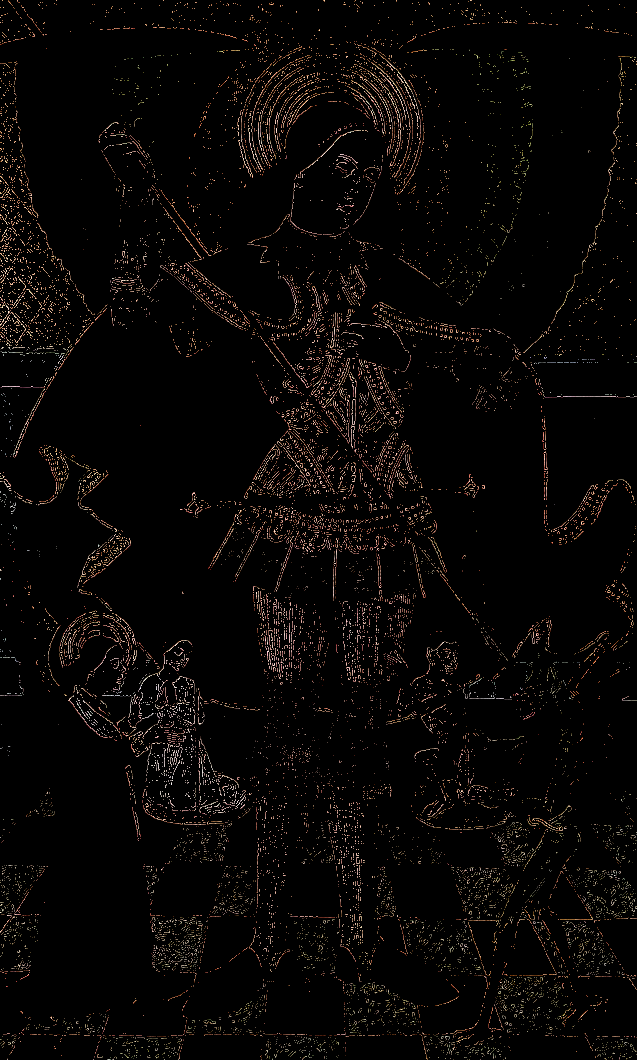
\includegraphics[angle=0,width=0.45\textwidth]{afsnit/afprovning/billeder/thressholds/krafitige_farver/krafite_detalier/1_iteration/500-500.png}
        \label{500-500}}\hspace{1em}
    \subfloat[600,600]{
        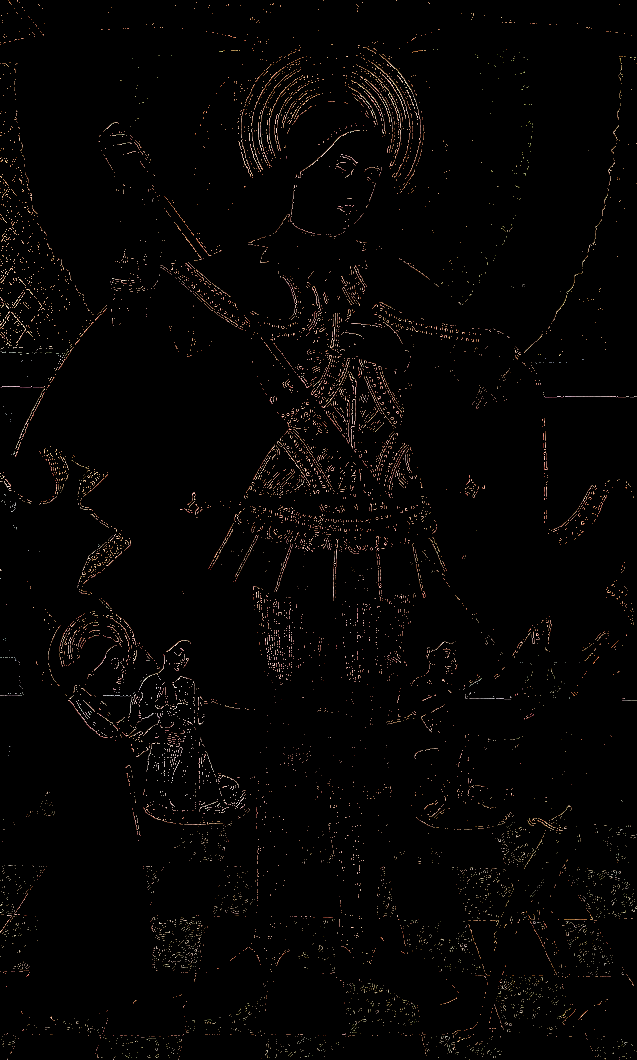
\includegraphics[angle=0,width=0.45\textwidth]{afsnit/afprovning/billeder/thressholds/krafitige_farver/krafite_detalier/1_iteration/600-600.png}
        \label{600-600}}\\
    \subfloat[700,700]{
        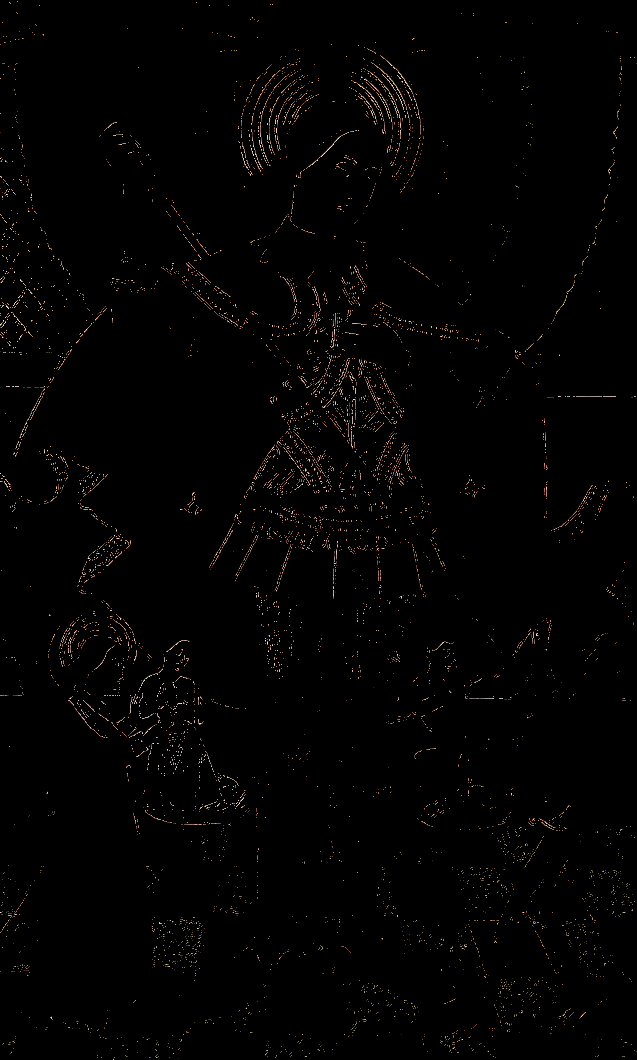
\includegraphics[angle=0,width=0.45\textwidth]{afsnit/afprovning/billeder/thressholds/krafitige_farver/krafite_detalier/1_iteration/700-700.png}
        \label{700-700}}\hspace{1em}
    \subfloat[Original]{
        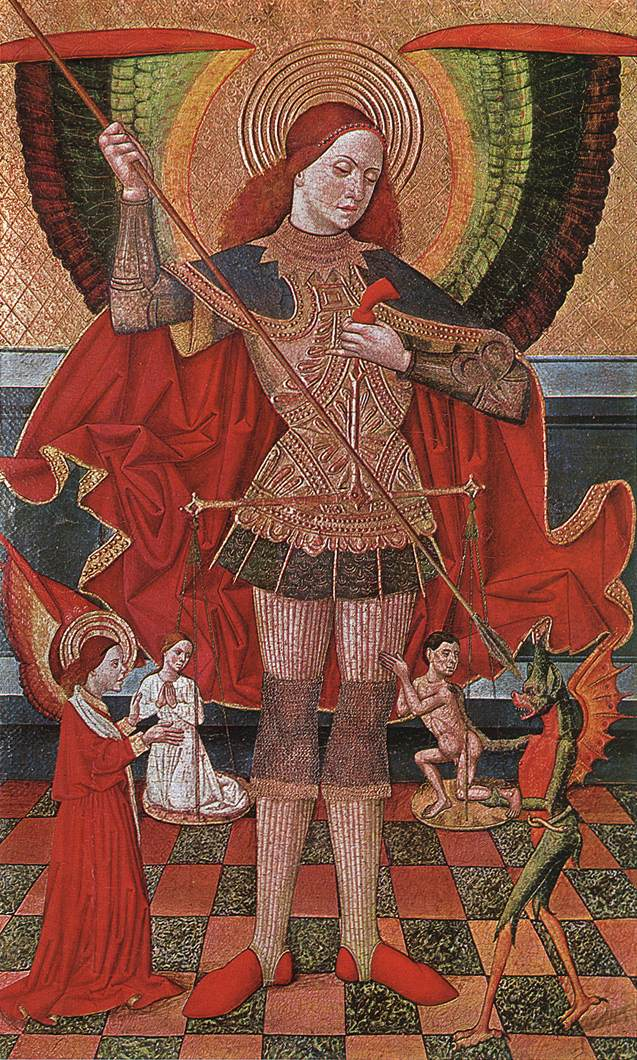
\includegraphics[angle=0,width=0.45\textwidth]{afsnit/afprovning/billeder/thressholds/krafitige_farver/krafite_detalier/kDetalier.jpg}
        \label{kDetalier}}
    \caption[]{Edgedetection på maleriet \ref{kDetalier} som har mange detaliger og kraftige farver, med tærskelværdierne fra 100-100 til 700-700}
    \label{allesammen2}
\end{figure}
\begin{figure}[!h]
    \centering
    \subfloat[300,700]{
        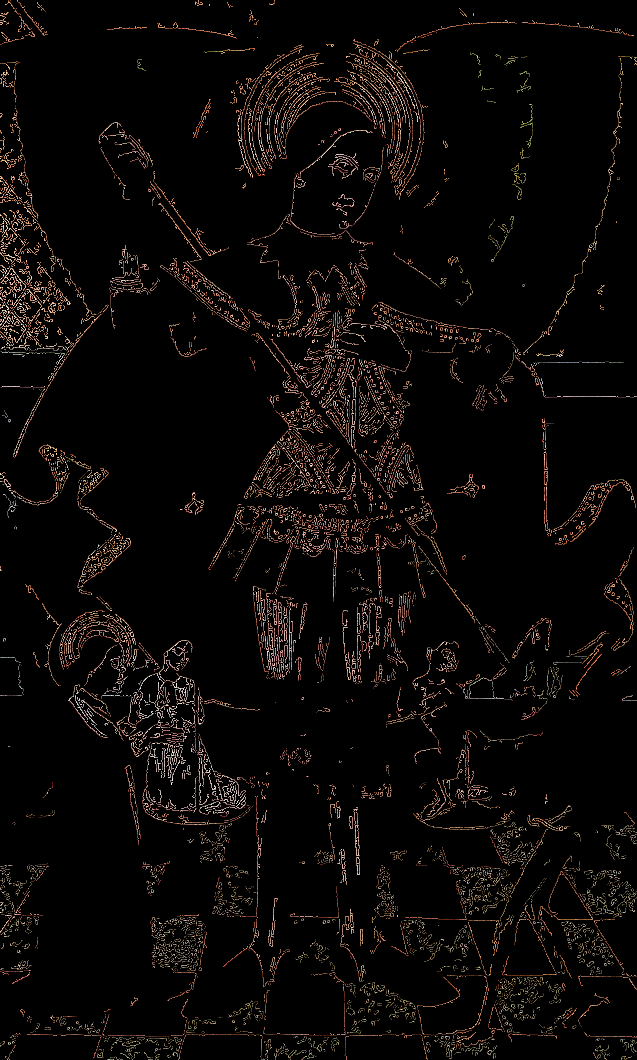
\includegraphics[angle=0,width=0.45\textwidth]{afsnit/afprovning/billeder/thressholds/krafitige_farver/krafite_detalier/2_iteration/300-700.png}
        \label{300-700}}\hspace{1em}
    \subfloat[300,750]{
        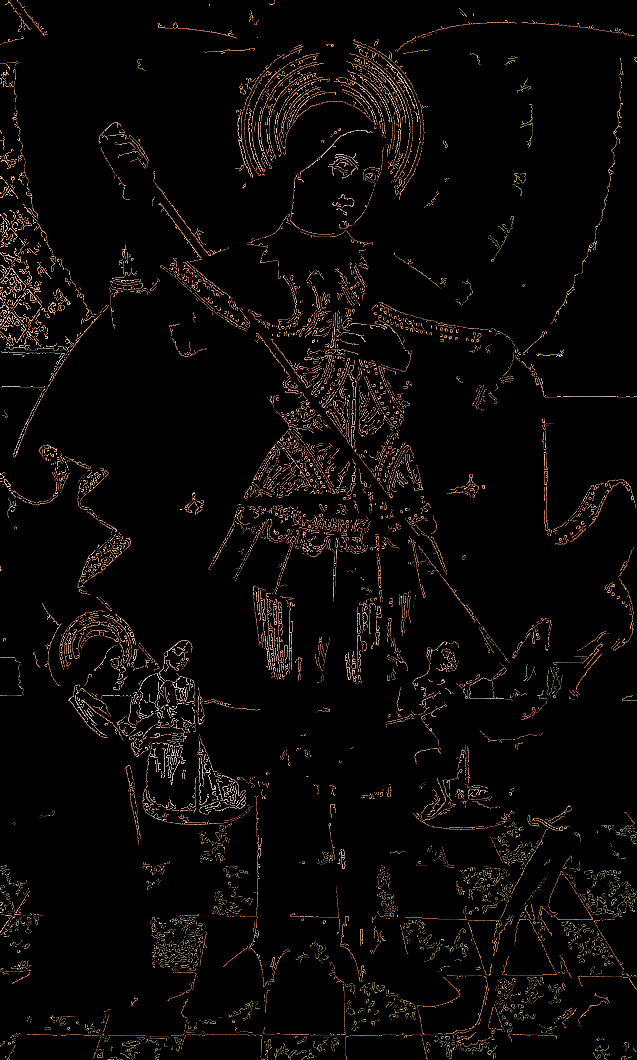
\includegraphics[angle=0,width=0.45\textwidth]{afsnit/afprovning/billeder/thressholds/krafitige_farver/krafite_detalier/2_iteration/300-750.png}
        \label{300-750}}\\
    \subfloat[300,800]{
        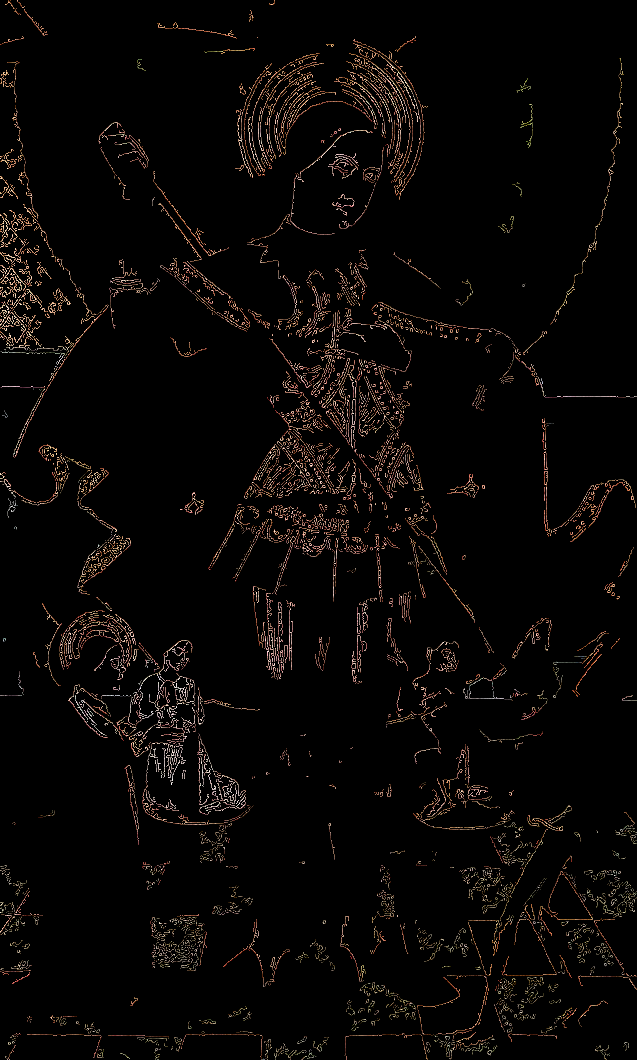
\includegraphics[angle=0,width=0.45\textwidth]{afsnit/afprovning/billeder/thressholds/krafitige_farver/krafite_detalier/2_iteration/300-800.png}
        \label{300-800}}\hspace{1em}
    \subfloat[300,850]{
        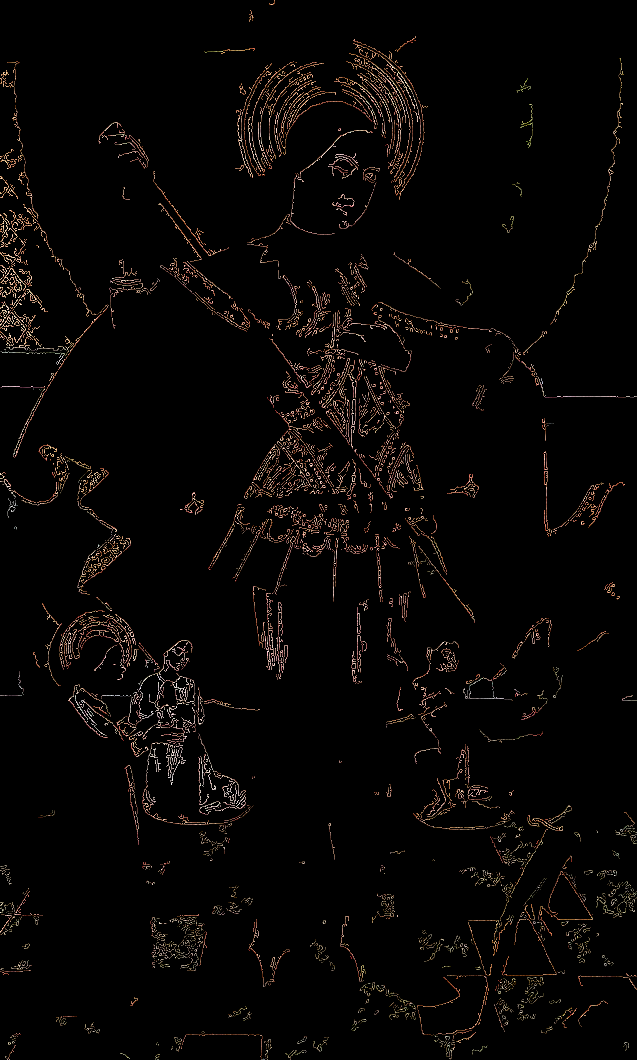
\includegraphics[angle=0,width=0.45\textwidth]{afsnit/afprovning/billeder/thressholds/krafitige_farver/krafite_detalier/2_iteration/300-850.png}
        \label{300-850}}\\
        \caption[]{Edgedetection hvor de 4 billeder som er intrasante taget med}
     \label{allesammen3}
\end{figure}
 
\begin{figure}[!h]
    \centering
    \subfloat[100,250]{
        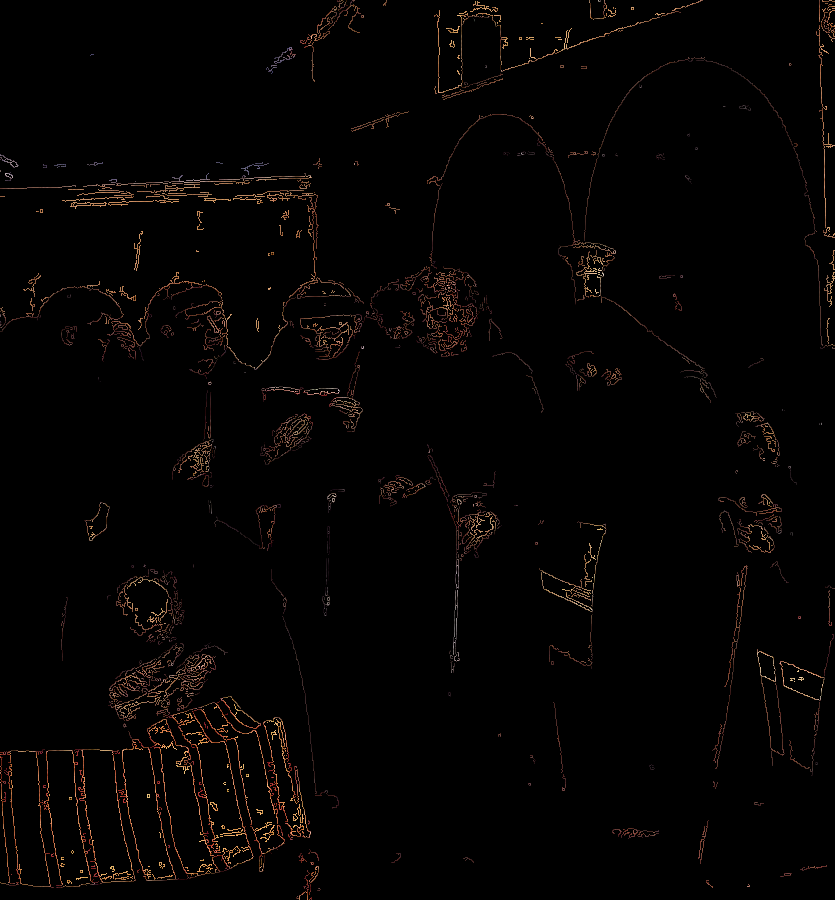
\includegraphics[angle=0,width=0.45\textwidth]{afsnit/afprovning/billeder/thressholds/svage_farver/svage_detalier/2_iteration/100-250.png}
        \label{100-250}}\hspace{1em}
    \subfloat[Orginal]{
        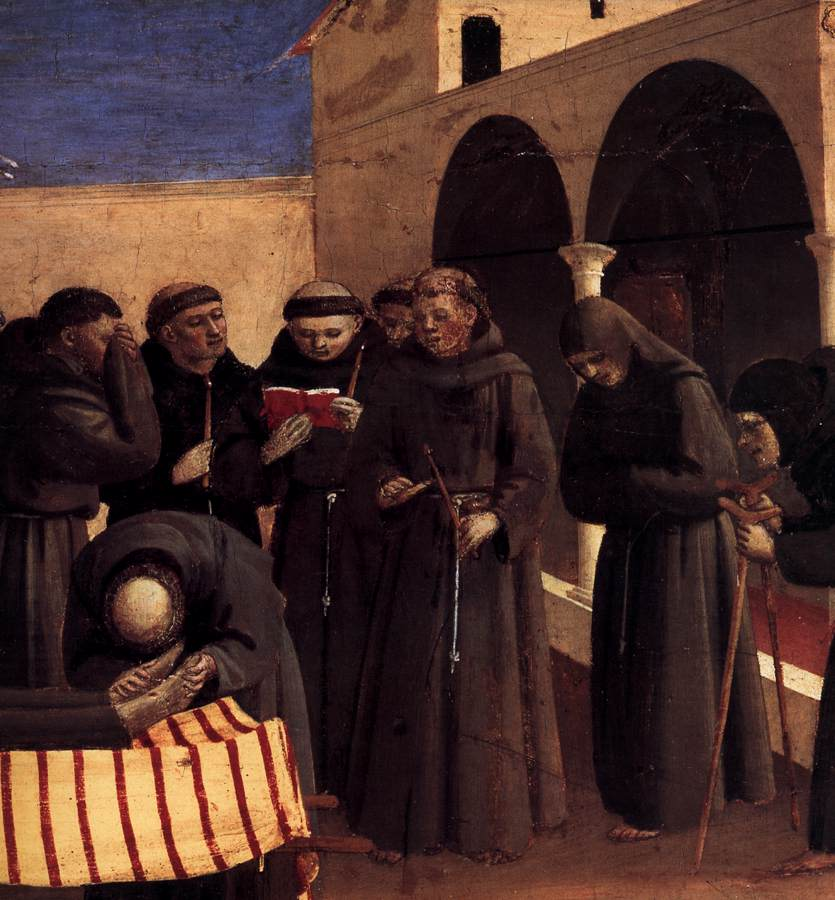
\includegraphics[angle=0,width=0.45\textwidth]{afsnit/afprovning/billeder/thressholds/svage_farver/svage_detalier/sDetalier.jpg}
        \label{Orginal}}\\
        \caption[]{Edgedetection på et billedet med svage farver og få detalier, hvor tærskenværdigern [100,250] er den beste}
     \label{1}
\end{figure}

\begin{figure}[!h]
    \centering
    \subfloat[100,240]{
        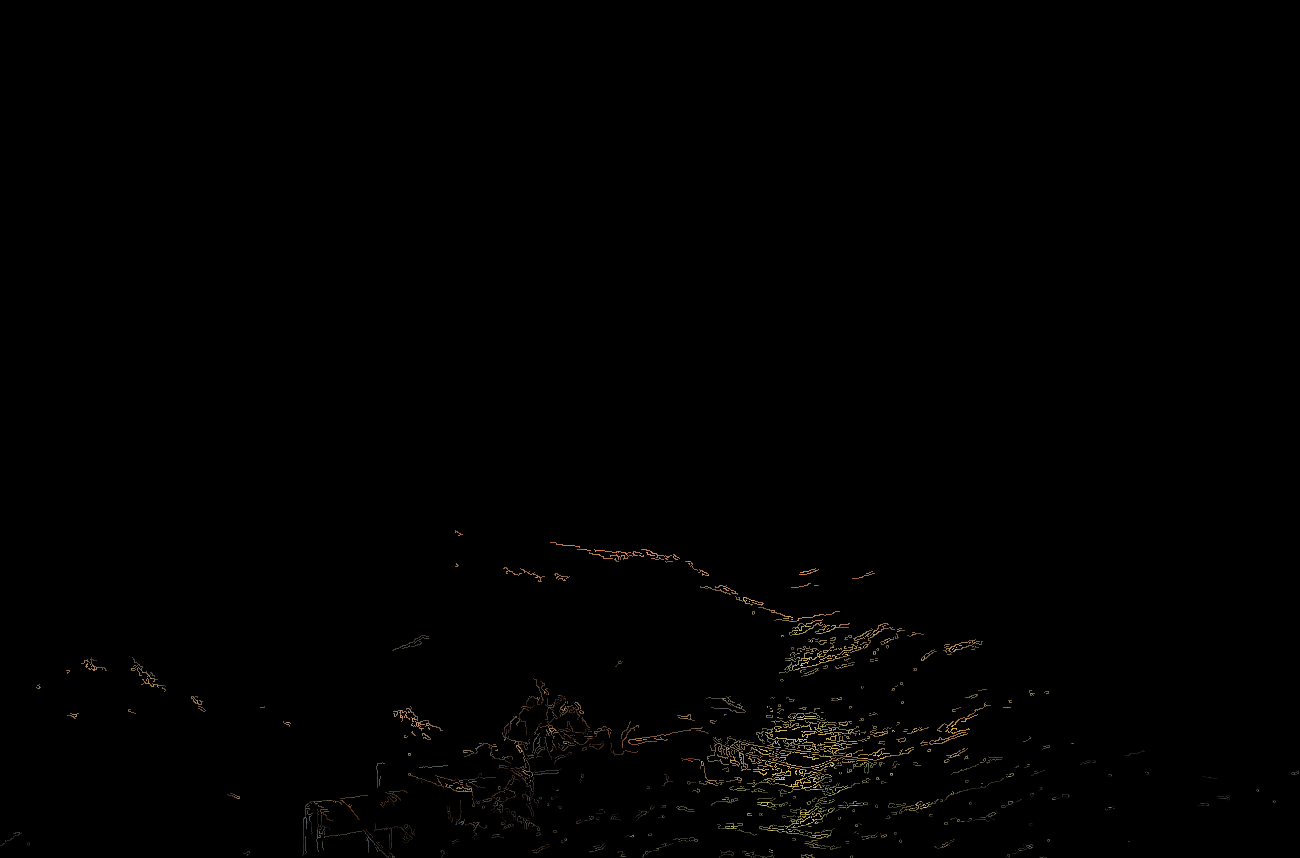
\includegraphics[angle=0,width=0.45\textwidth]{afsnit/afprovning/billeder/thressholds/medium_farver/svage_detalier/2_iteration/100-240.png}
        \label{100-240}}\\
    \subfloat[Orginal]{
        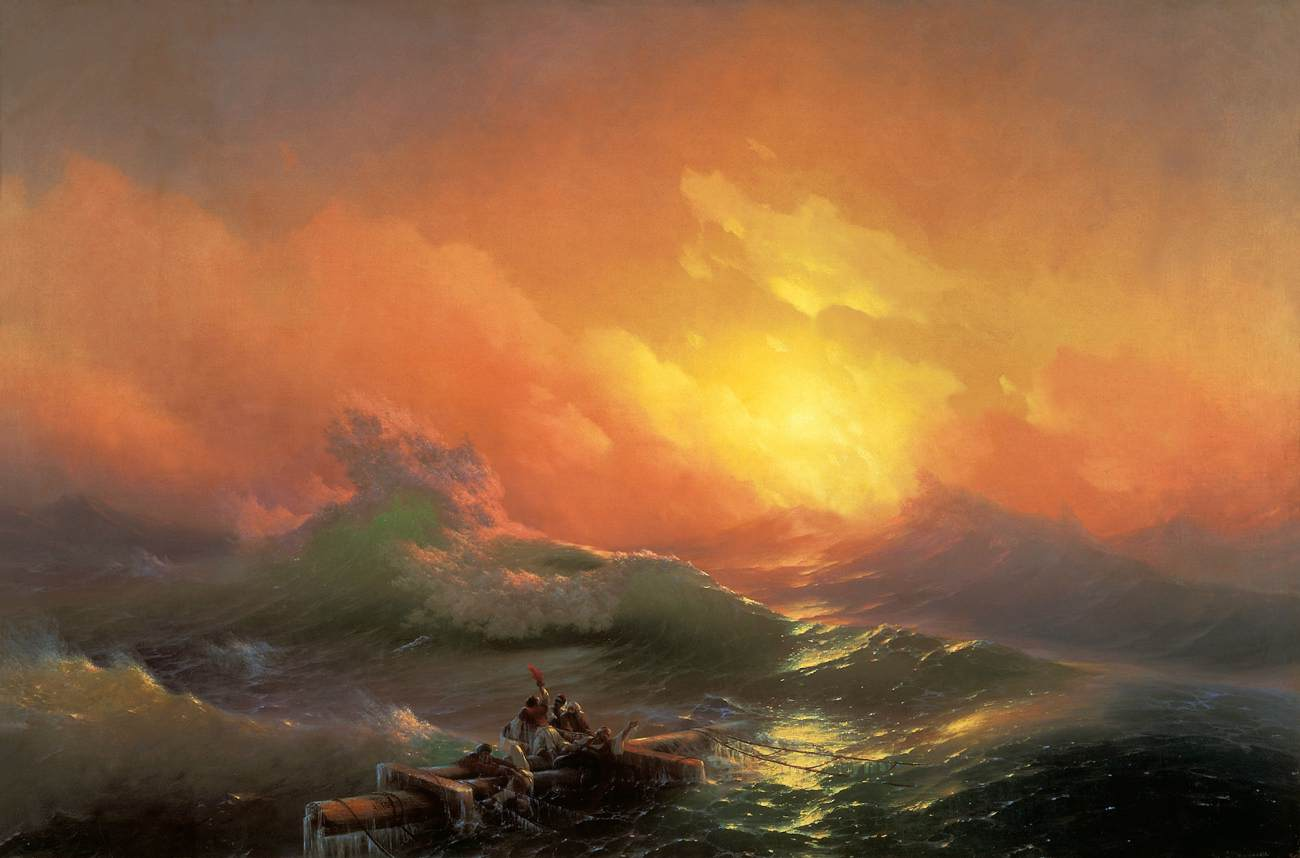
\includegraphics[angle=0,width=0.45\textwidth]{afsnit/afprovning/billeder/thressholds/medium_farver/svage_detalier/sDetalier1.jpg}
        \label{Orginal}}\\
        \caption[]{Edgedetection på et billedet med medium farver og få detalier, hvor tærskenværdigern [100,240] er den beste}
     \label{2}
\end{figure}


\subsubsection{Krafige farver og medium detalier}
\subsubsection{Krafige farver og få detalier}
\subsubsection{Medium farver og mange detalier}
\subsubsection{Medium farver og medium detalier}
\subsubsection{Medium farver og få detalier}
\subsubsection{Svage farver og mange detalier}
\subsubsection{Svage farver og medium detalier}
\subsubsection{Svage farver og få detalier}










threshold1,threshold2 = 78, 156
threshold1,threshold2 = 78, 156







